%-------------------------------------------------------------------------------
% seq66_patterns_panel
%-------------------------------------------------------------------------------
%
% \file        seq66_patterns_panel.tex
% \library     Documents
% \author      Chris Ahlstrom
% \date        2015-08-31
% \update      2018-10-27
% \version     $Revision$
% \license     $XPC_GPL_LICENSE$
%
%     Provides the concepts.
%
%-------------------------------------------------------------------------------

\section{Patterns Panel}
\label{sec:seq66_patterns_panel}

   \textsl{Sequencer66} works with patterns (loops, tracks, or
   sequences) that are repeated throughout a song.
   One composes and edits small patterns,
   and combines them to create a full song.  This is a powerful way
   to work, and makes one productive within an hour.

   The \textsl{Sequencer66 Patterns Panel} is the
   \index{main window}
   \textbf{main window} of \textsl{Sequencer66}.
   See \figureref{fig:seq66_main_screen}.
   It is called the "main window" or the "patterns window".
   It is here one creates a set of patterns
   (see \sectionref{subsubsec:concepts_terms_screen_set}),
   manages the configuration, controls the playback rate, adds tempo events,
   and opens the pattern, song, event, or playlist editors.

   \index{live mode}
   \index{mode!live}
   \index{mode!song}
   When the Patterns Panel has the application focus,
   and \textsl{Sequencer66} is \textsl{not} running in \textbf{Song} mode,
   it puts \textsl{Sequencer66} in \textbf{Live} mode.
   The musician can
   control the playback and muting/unmuting of each pattern in
   the song, while it is playing, from within this window.

   \index{song mode}
   \index{mode!song}
   If the song editor (see \sectionref{sec:seq66_song_editor})
   has the input focus, it controls the muting/unmuting of
   each pattern, and \textsl{Sequencer66} runs in \textbf{Song} mode.
   (There are ways to override this behavior.)

%  However, if \textsl{Sequencer66} is using JACK transport, then, instead of
%  the behavior described above, live versus song mode is controlled by the
%  JACK start mode option (see the \textbf{JACK Start mode} item in
%  \sectionref{paragraph:seq66_menu_file_options_jack_sync}).

   For exposition, we break the Patterns Panel
   into a menu bar, a top panel, a pattern panel, and a bottom panel.
   The \textsl{Sequencer66} menu bar is discussed in
   \sectionref{sec:seq66_menu}.
   The Qt and Gtkmm user-interfaces differ in the arrangement of buttons and
   panels; and the Qt interface uses tabs.

\subsection{Patterns / Top Panel}
\label{subsec:seq66_patterns_panel_top}

   The top panel of the Pattern window is simple, consisting of the
   name of the program and a few controls.  The latest version adds more
   buttons.
   
%  The original version looked like
%  this:

% \begin{figure}[H]
%    \centering 
%    \includegraphics[scale=0.75]{pattern-window-top-panel-items.png}
%    \caption{Patterns Panel, Top Panel, Older Version}
%    \label{fig:pattern_window_top_panel_items}
% \end{figure}

%  But, if compiled with \texttt{SEQ64\_STAZED\_MENU\_BUTTONS} defined,
%  there are some extra buttons available:

\begin{figure}[H]
   \centering 
%  \includegraphics[scale=0.50]{pattern-window-top-panel-items-new.png}
%  \includegraphics[scale=0.50]{new/pattern-window-top-panel-items-new.png}
%  \includegraphics[scale=0.50]{new/pattern-window-top-panel.png}
%  \includegraphics[scale=0.75]{new/pattern-window-top-panel.png}
   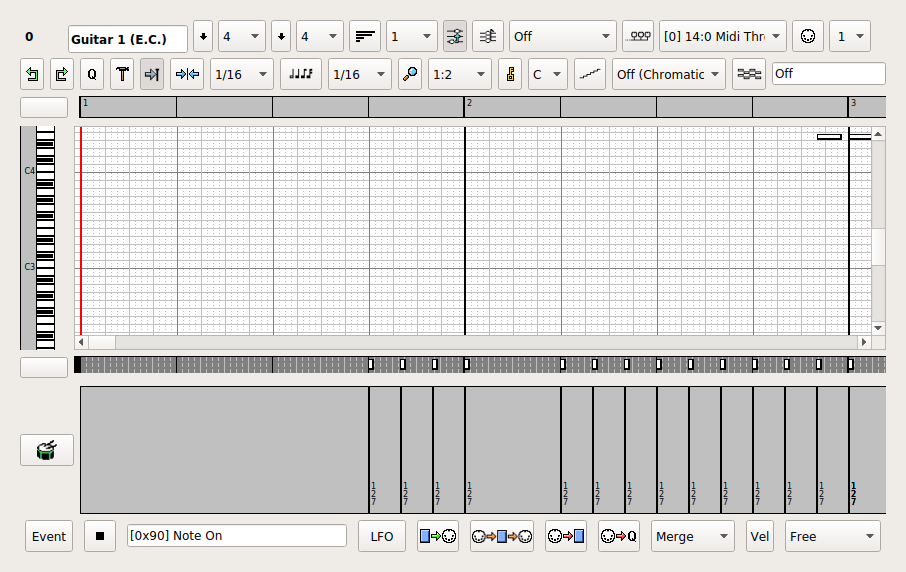
\includegraphics[scale=0.65]{roll.png}
   \caption{Patterns Panel, New Top Panel Items}
   \label{fig:pattern_window_new_top_panel_items}
\end{figure}

   This figure shows the appearance of the main window top panel.
   These items appear in the Gtkmm-2.5 user-interface.
   The Qt user-interface is arranged differently, but has roughly the
   same functionality.
   See \figureref{fig:seq66_main_screen_qt}.

%  If \textsl{Sequencer66} was built with
%  \texttt{SEQ64\_MENU\_BUTTON\_PIXMAPS} defined, then the buttons have icons
%  on them; otherwise they have text.  The figure shows what they look like,
%  and how they look with the song/live and toggle-menu functions activated.
 
   \begin{enumber}
      \item \textbf{Song/Live}
      \item \textbf{Toggle Playing Tracks}
      \item \textbf{Toggle Menu}
      \item \textbf{ALSA/JACK Modes}
      \item \textbf{Song Progress Bar}
      \item \textbf{Time Display Selection}
      \item \textbf{Mute Group Learn}
   \end{enumber}

   \setcounter{ItemCounter}{0}      % Reset the ItemCounter for this list.

   \itempar{Song/Live}{pattern!song/live}
   \index{pattern!song/live}
   This new button allows the Song mode to be in force even if
   the \textbf{Song Editor} does not have the focus of the application.
   However, if the \textbf{Song Editor} does have focus, it overrides this
   button, to preserve expected behavior.
   There is also a configurable hot-key associated with it,
   which defaults to \texttt{F1}, and is configurable in the "rc" file and
   the \textbf{File / Options / Ext Keys} page.

   \itempar{Toggle Tracks}{pattern!toggle tracks}
   \index{pattern!toggle tracks}
   This button changes the status of all of the
   \textsl{playing} tracks, reversing the
   mute status of each pattern that is playing.
   The next click will then unmute only those tracks.
   Because it can be confusing, this button is disabled (not shown
   in the figure) in Song mode.
   There is also a configurable hot-key associated with it, called
   \textbf{Toggle mutes},
   which defaults to \texttt{F8}, and is configurable in the "rc" file and
   the \textbf{File / Options / Ext Keys} page.

   \itempar{Toggle Menu}{pattern!toggle menu}
   \index{pattern!toggle menu}
   This button enables and disables the main menu.
   Disabling it allows additional hot-keys to be configured,
   without calling forth menu entries by accident.
   There is also a configurable hot-key associated with this toggle, called
   \textbf{Menu mode},
   which defaults to \texttt{F3}, and is configurable in the "rc" file and
   the \textbf{File / Options / Ext Keys} page.

   \itempar{ALSA/JACK Modes}{pattern!ALSA/JACK modes}
   \index{pattern!ALSA/JACK mode}
   This button sets the ALSA versus
   JACK modes, including JACK transport and native JACK MIDI playback and
   recording.
   When clicked, it brings up the JACK connection page from the
   \textbf{File / Options} dialog.  The hot-key for this button
   is \texttt{Ctrl-P}.

   \itempar{Song Progress Bar}{pattern!progress bar}
   \index{pattern!progress}
   \index{pattern!"main time"}
   The \textbf{Song Progress Bar} is also known as the "main time" bar.
   Also included is a numeric representation of the "BBT" (bar:beat:ticks).
   In the Gtkmm-2.4 user-interface,
   this bar shows a number of small black cursors ("pills") that show the
   progress of the song through the various patterns.  For short patterns,
   the progress is fast.  For patterns that last longer, the progress is
   slow.  The whole field flashes in time with the beat.
   This field shows that something is going on.  It can also indicate
   the relative lengths of the various patterns.
   In the Qt user-interface, this bar is shown as four boxes
   which blink in time with playback.
 
   Note that the individual pattern boxes in the main panel, for
   patterns that are not empty, have their own
   moving progress cursor, a vertical line in each box.
   By default, this progress line is black, but it can be changed to
   other colors via a "user" configuration file entry in the 
   \texttt{[user-interface-settings]} section.
   Set the \texttt{progress\_bar\_colored} item to a value ranging from 0
   (black) to 6 (dark cyan).
   There is also a \texttt{progress\_bar\_thick} item to enable a thicker
   progress bar, for better visibility.

%  Even if not enabled, the currently-selected pattern will show as highlighted
%  in dark-cyan.

   \itempar{Time Display Selection}{pattern!time display}
   The \textbf{Time Display Selection} is also known as the "main time" bar.
   This button toggles between the states of \textbf{BBT} (bar:beats:ticks)
   and \textbf{HMS} (hours:minutes:seconds).

   \itempar{Mute Group Learn}{pattern!mute group learn}
   \index{L button}
   \index{"L" button}
   This button is also known as the "L" button.
   Click this button, and then press a mute-group key
   to store the mute-state (whether armed or unarmed)
   of all the patterns with in that key.
   In addition to this button, one can also press
   the \texttt{Ctrl-L} key.
%  (analogous to the \texttt{Ctrl-E}
%  keystroke that brings up the Song Editor).
   \index{auto-shift}
   \index{group-learn!auto-shift}
   \index{shift-lock}
   \index{group-learn!shift-lock}
   When in group-learn mode, the \texttt{Shift} key cannot be hit, so the
   group-learn mode automatically converts the keys to their shifted versions.
   This feature known as \textsl{shift-lock} or \textsl{auto-shift}.

   See the \textbf{File / Options / Keyboard} menu entry for the
   dialog showing the available mute-group keys and the corresponding
   hot-key for the "L" button.
   This key is usually the \texttt{Insert} key.  Unlike the button or the
   \texttt{Ctrl-L} key, this key must be held down while pressing the desired
   mute-group key.
   This is a clumsy thing on our main keyboard... one must press and hold
   \texttt{Shift-Fn-Insert} to get the \texttt{Insert} key, and then also
   press the desired mute-group key.  A real knuckle-buster!
   We have our own alternate setup (stored in the file
   \texttt{sequencer66.rc.example}.
   And we've also added the "shift-lock" feature for this reason.

   Group-learn is a modifier key to be pressed
%  \textsl{together} with
   just before pressing
   the desired group key, and the group on/off keys are there to enable
   each group, \textsl{not} to toggle group states.

   To set up the mute groups, press the 'L' button, and then press a key on
   the keyboard to 'learn' or 'save' the preset. Looking at the list of keys
   assigned for these mute groups (in \textbf{File / Options / Keyboard}),
   the first bank of keys are "!", "'", "?", etc., and the second bank are
   "Q", "W" "E", etc.
%  Note that these shifted keys do not toggle patterns, but
%  set them to a saved mute-group of armed and unarmed patterns.
   If the key is valid, then the following prompt occurs:

\begin{figure}[H]
   \centering 
%  \includegraphics[scale=0.65]{pattern-window-group-learn-confirmation.png}
   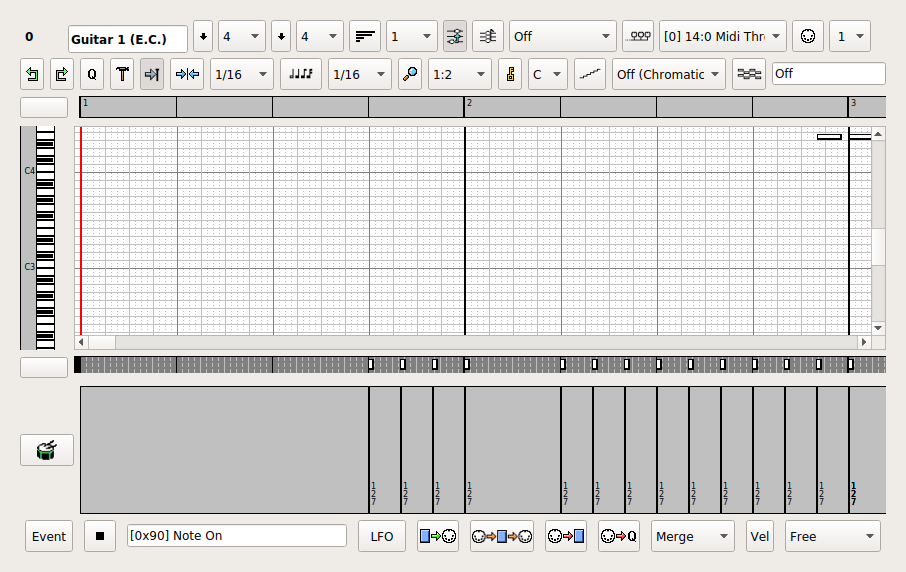
\includegraphics[scale=0.65]{roll.png}
   \caption{Group Learn Confirmation Prompt}
   \label{fig:pattern_window_group_learn_confirmation}
\end{figure}
   
   When you ask the program to 'learn' the key, one cannot
   use the Shift key, so one normally could not use the "!" or
   other symbol keys.
   In fact, the process stops as soon as the Shift key is pressed:

\begin{figure}[H]
   \centering 
%  \includegraphics[scale=0.65]{pattern-window-group-learn-failure.png}
   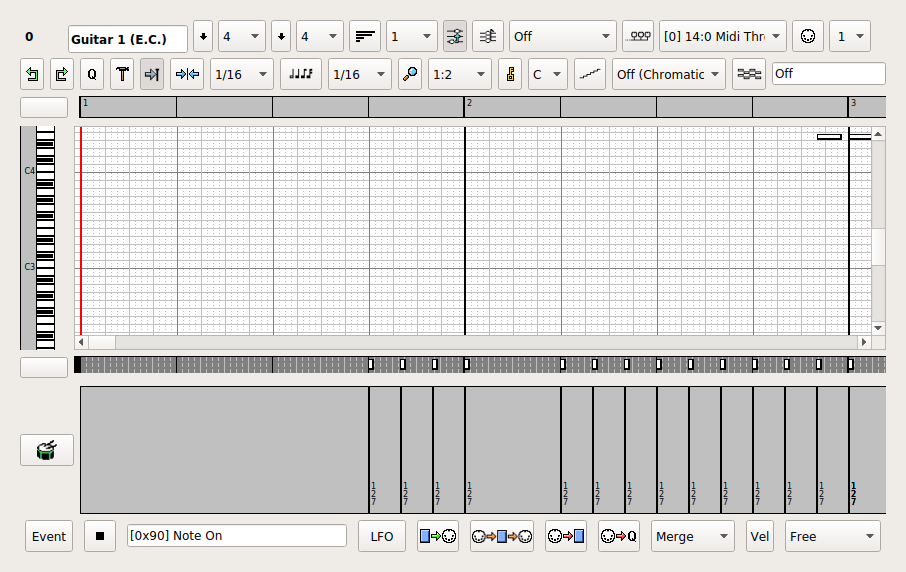
\includegraphics[scale=0.65]{roll.png}
   \caption{Group Learn Failure Prompt (Shift Key)}
   \label{fig:pattern_window_group_learn_failure}
\end{figure}

   \index{caps lock in learn mode}
   \index{auto-shift}
   \index{group-learn!auto-shift}
   \index{shift-lock}
   \index{group-learn!shift-lock}
   To avoid this issue with the \texttt{Shift} key, \textsl{Sequencer66} now
   "shift-locks" the keys while group-learn is in progress, so
   that none of the keys, whether letters or the punctuation characters above
   the numbers, need the \texttt{Shift} key to be held, to learn them.
   Thus, there is now no need to use the \textbf{Caps Lock} is \textsl{On} before
   starting the "learn" process.  We tend to map the
   \texttt{Caps Lock} key as the \textsl{true} Control key, so that
   \texttt{Caps Lock} is no longer available anyway
   (it is one of the most useless keys \textsl{ever}).

   Remember, though, that once learned, the \texttt{Shift} is then
   needed to call up the mute-group that was learned.

   There is another way for mute-group learn to fail.
   With the recent ability of \textsl{Sequencer66} to increase the set size via
   the \texttt{--option sets=8x12} (for example), there can be fewer than 32
   mute-groups available.   This can be seen by viewing
   \textbf{File / Options / Keyboard} when larger set-sizes are in force:

\begin{figure}[H]
   \centering 
%  \includegraphics[scale=0.75]{group-learn-limited.png}
   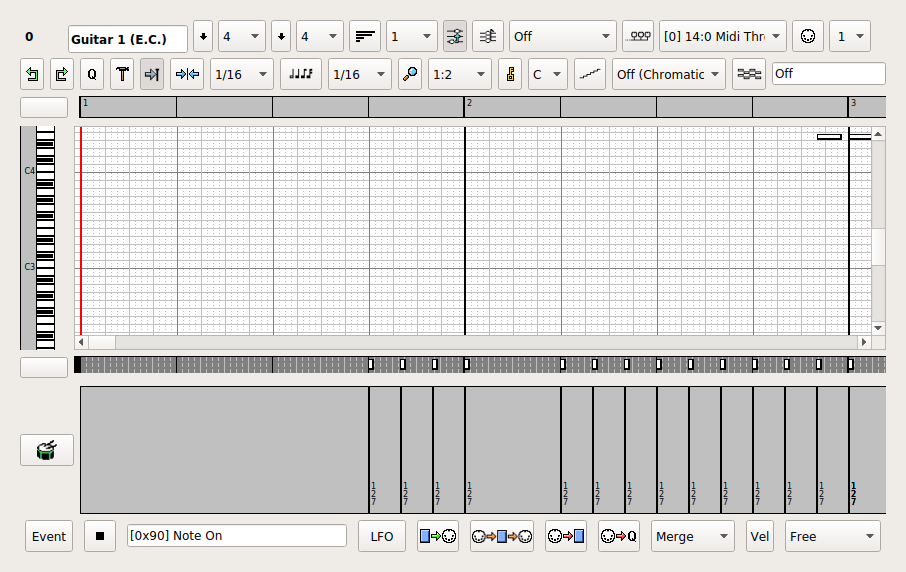
\includegraphics[scale=0.65]{roll.png}
   \caption{Group Learn Keys With Larger Set Size}
   \label{fig:pattern_window_group_learn_limited}
\end{figure}

   Note that only 10 mute-groups (0 to 9) are available with an 8x12 set size.
   Groups 10 and above are not available, and this is indicated by the word
   "Clear".  Don't worry, though, all of the mute-group key settings still
   exist, and are still present in the "rc" configuration file in the
   \texttt{[keyboard-group]} section.

   But when one attempts a group-learn using one of the unavailable keys,
   an error occurs, as shown in the following prompt.

\begin{figure}[H]
   \centering 
%  \includegraphics[scale=0.75]{pattern-window-group-learn-limit.png}
   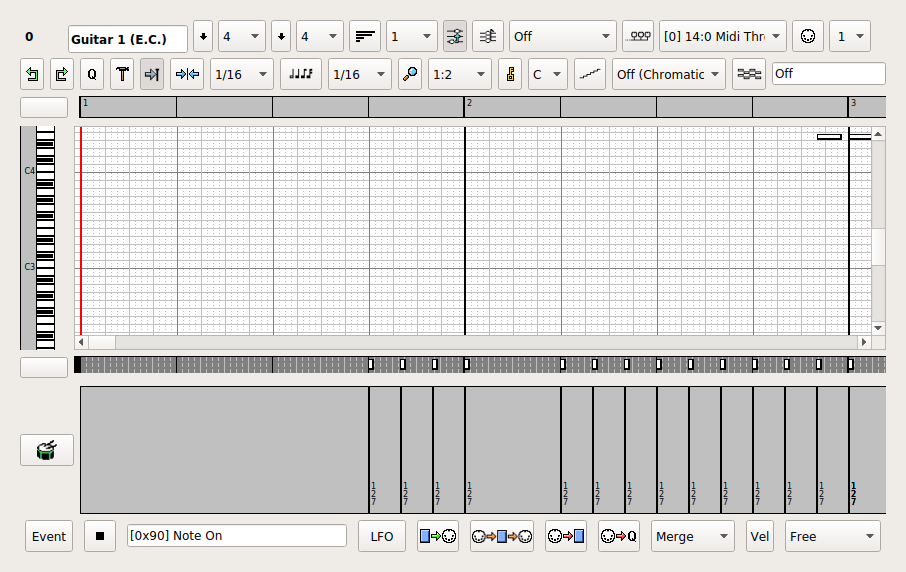
\includegraphics[scale=0.65]{roll.png}
   \caption{Group Learn Limit Prompt}
   \label{fig:pattern_window_group_learn_limit}
\end{figure}

   This prompt also appears if one tries to use the shifted version of an
   unavailable mute-group key to toggle patterns; this makes it obvious what
   has gone wrong.

   \textsl{
   At some point in the future, we may allow a much larger number of sets, so
   that all 32 mute-groups are always available.  We have to think hard about
   that enhancement, however.
   }

   One can configure the MIDI settings in similar ways
   by assigning MIDI commands to arm or toggle loops, using 
   \index{rc file}
   the 'on' option in the "rc" file.
   See \sectionref{subsec:seq66_rc_file_midi_control}.

%  The mute group doesn't toggle... it turns on.
%  \index{group!toggle}
%  \index{group!arm}
%  \index{group!unmute}
%  One can toggle the playing status of up to 32 previously
%  One can set the playing status of up to 32 previously
%  defined mute/unmute patterns (groups) in the active screenset, similar to
%  hardware sequencers.  One can mute-unmute (according to the group
%  definition) all loops in the playing screenset, which is the only one that
%  can have sequences playing if a mute group is selected
%  (like a live sequencer).
%
%  This arming is done either by one of the \textsl{group arm} keys
%  or by a MIDI controller, both assigned in the
%  \index{rc file}
%  \texttt{~/.config/sequencer66/sequencer66.rc} or \texttt{~/.seq24rc} files,
%  and easily modified in the \textbf{File / Options / Keyboard} tab.
%  These characters can be shown in each pattern (and in 0.9.11 and above, no
%  matter which screenset is active).
%
%  A mute/unmute pattern (group) is stored by holding a
%  \index{group!learn}
%  \textsl{group learn} key (\texttt{Insert} by default) while pressing the
%  corresponding \textsl{group arm} key.  The "L" button can also be used to
%  enter "Learn" mode.
%  Once a learn-key is pressed, the set of muted/unmuted patterns in the
%  current set is memorized, and can be recalled later.

%  There are also keys assigned to turn on/off the group functionality.

%  Once learned, the "Shifted" version of the keyboard keys can be
%  used to select a learned group.

   Remember that groups work with the playing ("in-view") screen-set.
   One must change the screenset and give it the command to make it the
   playing one.
   \index{keys!Home}
   By default, the \texttt{Home} key is configured for this purpose.

   So, for example, if one sets \texttt{A} to turn on the
   patterns in slots 1 and 2 in set 0 (the first set), then pressing
   \texttt{A} in another set will arm the patterns in the same relative
   location in the current set.
   This setup is flexible, but takes some thought.
   One can set up a number of mute-groups, and decide to use them
   for all sets, or mentally allocate one mute-group per set.
   Please note that a mute-group key does not \textsl{toggle} the saved
   armed patterns... it can only turn them on.

%  \index{rc file}
%  It is all configurable in the "rc" file.

   Let's go through an example using the \texttt{Home} key (or whatever key is
   configured as the \textbf{Set Playing Screenset} key.)

   \begin{enumber}
      \item Load a song with more than one screen-set.
      \item Unmute the pattern(s) in the first set and start playback.
      \item Use the "\texttt{]}" (\textbf{Screenset Up}) key to move to the next
         set.  Note that the first set is still playing.  Also note that the
         now-current set is \textsl{not} playing.
      \item Press the \texttt{Home} key.
         Note that the first set turns off, and the current set turns on.
         These steps can be repeated at will.
      \item Finally, hit the \texttt{F8} (\textbf{Toggle Mutes}) key.
         Note that all tracks on all sets toggle muting each time this key is
         pressed.
   \end{enumber}

\subsection{Patterns / Main Panel}
\label{subsec:seq66_patterns_panel_main}

   The main panel of the Patterns window provides a grid of empty boxes,
   each box delimited by brace-like lines at left and right.
   Each filled box represents a loop or pattern.
   One sees only 32 loops at a time in the main panel (but many more than
   32 loops can be supported by \textsl{Sequencer66}).
   \index{screen-set}
   This group of 32 loops is called a "screen-set", as discussed in
   \sectionref{subsubsec:concepts_terms_screen_set}.
   One can switch between sets by using the
   \index{keys![}
   \index{keys!screenset down}
   "\texttt{[}" and
   \index{keys!]}
   \index{keys!screenset up}
   "\texttt{]}" keys on the keyboard, or by using
   the spin-widget-driven, labelled \textbf{Set} interface item, or
   \index{keys!Home}
   \index{keys!screenset play}
   by hitting the (default) \texttt{Home} key to make it the playing screenset,
   or by hitting \texttt{Page-Up} or \texttt{Page-Down} with the pattern window
   in keyboard focus.
   There are a total of 32 sets, for a total of 1024 loops/patterns. 
   Only one screen-set can be controlled at a time, in general.
%  have found; have not yet tried to verify this assertion.
   But any number of screensets can be playing at the same time.

   Note that the \texttt{Page Up} and \texttt{Page Down} keystrokes, and their
   counterparts in
   \textbf{File / Options / Keyboard / Control Keys / Screenset Up}
   and \textbf{Screenset Down}, can be used in lieu of the
   \textbf{Set} spin-button.

   It is important to note that keystroke control of the screen-set will
   wrap-around in screen-set values (i.e. screen-set down at 0 results in
   screen-set 31, and screen-set up at 31 results in screen-set 0).
   However, the spinbuttons will stop up at 31 and stop down at 0.
   We consider this a feature rather than a bug, at this time.

\begin{figure}[H]
   \centering 
%  \includegraphics[scale=0.75]{pattern-window-main-panel-items.png}
   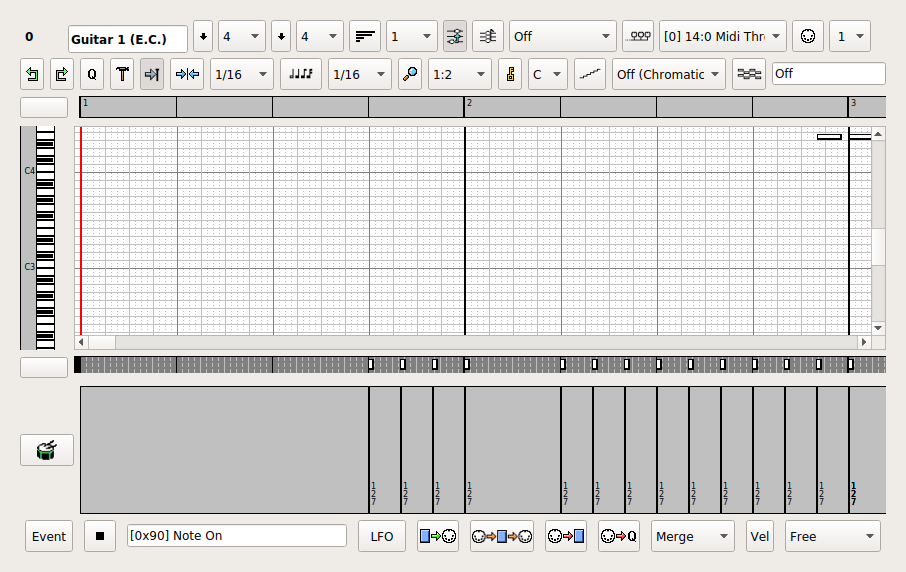
\includegraphics[scale=0.65]{roll.png}
   \caption{Patterns Panel, Main Panel Items}
   \label{fig:pattern_window_main_panel_items}
\end{figure}

   The individual items annoted in this figure are described in
   \sectionref{subsubsec:seq66_patterns_pattern_filled}, in more detail.
   The slot at the bottom left of this figure shows some new features:

   \begin{itemize}
      \item The sequence number appears at the bottom left of the slot.
      \item The buss number (re 0) and the channel number (re 1) appears
         to the right of the sequence number, in the format "0-1".
      \item To the right of that, the time signature ("4/4") appears, at the
         bottom.
      \item The hot-key for muting/unmuting the pattern appears next,
         at the bottom right of the slot.
      \item The title of the sequence appears at the top left of the pattern
         slot.
      \item The length of the sequence, in number of measures (bars), appears
         at the upper right of the slot.
      \item Notice the default alternate font, which has a little more body
         than the \textsl{Seq24} font.
   \end{itemize}

   Observe that feature in the first figure of the next section.
   The two main items are the empty \textsl{pattern slot}, and the slot filled
   with a MIDI \textsl{pattern}:

   \begin{enumber}
      \item \textbf{Pattern Slot}
      \item \textbf{Pattern}
   \end{enumber}

\subsubsection{Pattern Slot}
\label{subsubsec:seq66_patterns_pattern_slot}

   \index{pattern!slot}
   An empty box is a slot for a pattern.
   If a pattern is present in the slot, the top line will show
   the title of the pattern, and the number of measures in the pattern.
   The latter is not shown on some of the figures in this manual, a
   lack we will ave to rectify someday.
   Also, these colors are not yet supported in the Qt user-interface.

   A pattern can show a number of different statuses based on the coloring
   of elements in the pattern slot. 

\begin{figure}[H]
   \centering 
%  \includegraphics[scale=0.75]{new/slots.png}
   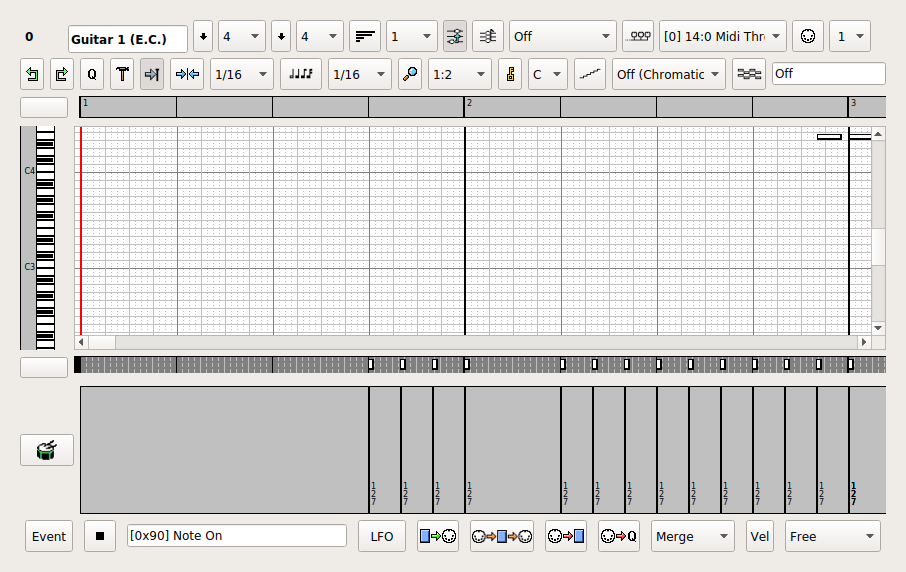
\includegraphics[scale=0.65]{roll.png}
   \caption{Various Status of Pattern Slots}
   \label{fig:pattern_slots_statuses}
\end{figure}

   Not shown in the figure are the gray pattern
   colors resulting from queuing and one-shot queuing, nor is the
   number-of-measures number shown.
   The colors have meaning (in the Gtkmm user-interface only):

   \begin{itemize}
      \item \textbf{Empty background}.  Whether the classic gray pattern
         of \textsl{Seq24}, or the many patterns of \textsl{Sequencer66},
         including all black with yellow sequence numbers, this
         slot coloring indicates that the slot is unused.
      \item \textbf{White background}.  Unarmed (muted) patterns show black
         text on a white background.
      \item \textbf{Black background}.  Armed (unmuted) pattern.  If the text
         is yellow, it is a pattern with no MIDI events, but is armed.  Note
         that armed/unmuted patterns can be exported if they have a layout in
         the Song Editor.
      \item \textbf{Yellow background}.  A pattern with no MIDI events, just
         textual MIDI information.  If armed (uselessly), it is yellow text on
         a black background (not shown).
      \item \textbf{Cyan background, black text}.
         An unarmed pattern currently being edited in a 
         \textbf{Pattern Editor} or event
         editor. Or, if an SMF 0 MIDI file was just opened or imported, this
         color combination indicates the SMF 0 format track with all of the
         data in the song, which only occurs in slot 16 (unless the user then
         dragged it to another slot).
      \item \textbf{Black background, cyan text}.
         An armed pattern currently being edited in a 
         \textbf{Pattern Editor} or event
         editor.  Or an armed SMF 0 format MIDI sequence.
      \item \textbf{Red events}.
         Indicates a pattern for which the new transpose feature is
         disabled.  The white, black, and cyan background have the same
         meanings as in the other items for statuses of unarmed, armed, and
         currently being edited.
   \end{itemize}

   As of version 0.95, the user can also apply coloring to each sequence.
   This feature was adopted from \textsl{Kepler34} (\cite{kepler34}).
   Here is the new pattern menu for sequence color:
   \index{pattern!color menu}

\begin{figure}[H]
   \centering 
%  \includegraphics[scale=0.75]{new/seq66-sequence-color-menu.png}
   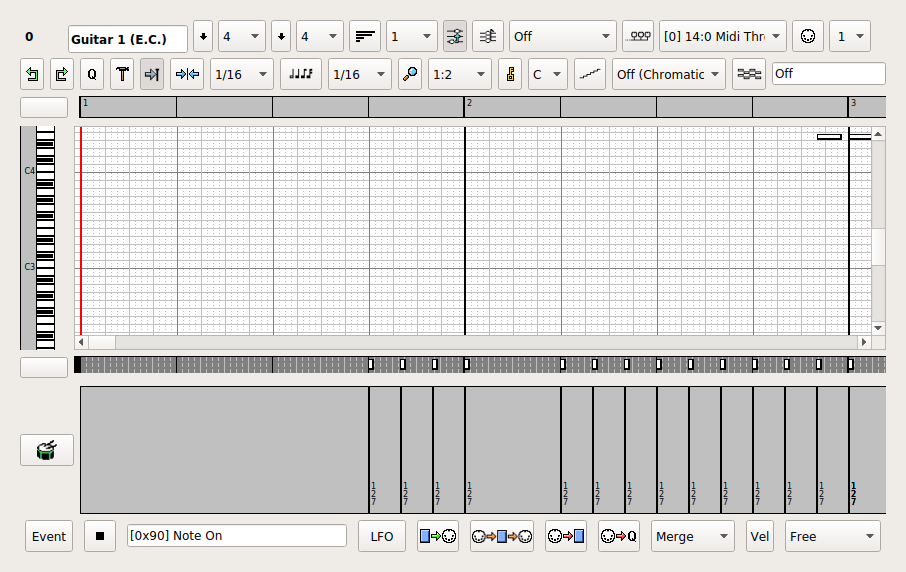
\includegraphics[scale=0.65]{roll.png}
   \caption{Sequence/Pattern Color Menu}
   \label{fig:pattern_window_sequence_color_menu}
\end{figure}

   Here is a sample of the coloration as it appears in the patterns panel and
   in the song editor:
   \index{pattern!coloring}

\begin{figure}[H]
   \centering 
%  \includegraphics[scale=0.75]{new/seq66-sequence-coloration.png}
   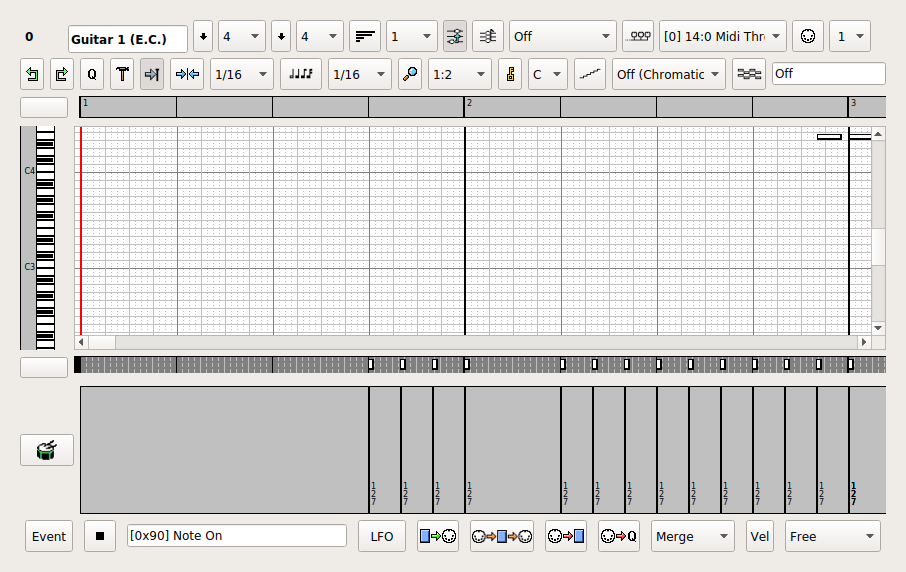
\includegraphics[scale=0.65]{roll.png}
   \caption{Sequence/Pattern Coloration}
   \label{fig:pattern_window_sequence_coloration}
\end{figure}

   \index{pattern!right click}
   \index{slot!empty slot right-click}
   Right-click on an empty box one brings up a menu to create
   a new loop, as well as some other operations:

\begin{figure}[H]
   \centering 
%  \includegraphics[scale=0.75]{pattern/pattern-empty-right-click-menu.png}
%  \includegraphics[scale=0.65]{new/pattern-empty-right-click-menu.png}
   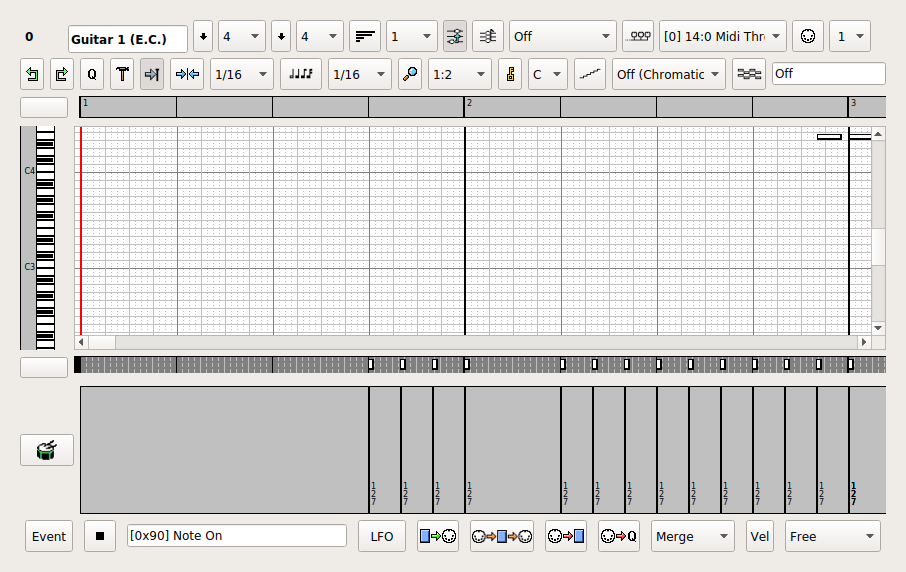
\includegraphics[scale=0.65]{roll.png}
   \caption{Empty Pattern, Right-Click Menu}
   \label{fig:pattern_window_empty_right_click}
\end{figure}

   \begin{enumber}
      \item \textbf{New}
      \item \textbf{Paste}
      \item \textbf{Song}
      \begin{itemize}
         \item {Mute All Tracks}
         \item {Unmute All Tracks}
         \item {Toggle All Tracks}
         \item {Toggle Live Tracks}
      \end{itemize}
   \end{enumber}

   This menu entry is quite different for the Qt user-interface.
   See \sectionref{subsubsec:qt_portmidi_qt5_live_slot_menu}.

   \setcounter{ItemCounter}{0}      % Reset the ItemCounter for this list.

   \itempar{New}{pattern!new}
   Creates a new loop or pattern.
   Clicking this menu entry fills in the empty box with an untitled
   pattern, and brings up the Pattern Editor
   so that one can fill in the new pattern.

   In addition to right-click and select \textbf{New}, the user can
   \index{empty slot double-click}
   double-click on the empty slot, to bring up a new instance of the sequence
   editor.  For the double-click, the effect can be a bit confusing at first,
   because it also toggles the arming/mute status of the slot
   quickly twice (leaving it as it was).  It takes some getting
   used to, but we miss it when using \textsl{Seq24}.

   \index{editing shortcut}
   \index{keys!=}
   \index{keys!pattern edit}
   \index{keys!-}
   \index{keys!event edit}
   A nice feature is hitting the equals ("=") key, then hitting
   a pattern shortcut key (hot-key), to bring up a new sequence or edit an
   existing one in a 
   \textbf{Pattern Editor} .  Another feature is hitting the minus
   ("-") key, then the hot-key, to bring up the \textbf{Event Editor}.
   The configuration file settings for the the '=' and
   '-' keys can be altering in the \textbf{File / Options / Keyboard} tab.

   \index{current slot highlight}
   When an unarmed (muted) pattern is first brough up for sequence editing (or
   event editing), the slot in the main window is now highlighted (Gtkmm only),
   using black text on a cyan background, as being the "currently-edited" slot.
   (This is the same background used to indicate the original track in an
   SMF 0 to SMF 1 conversion.)

\begin{figure}[H]
   \centering 
%  \includegraphics[scale=0.75]{pattern-window-current-seq-unarmed.png}
   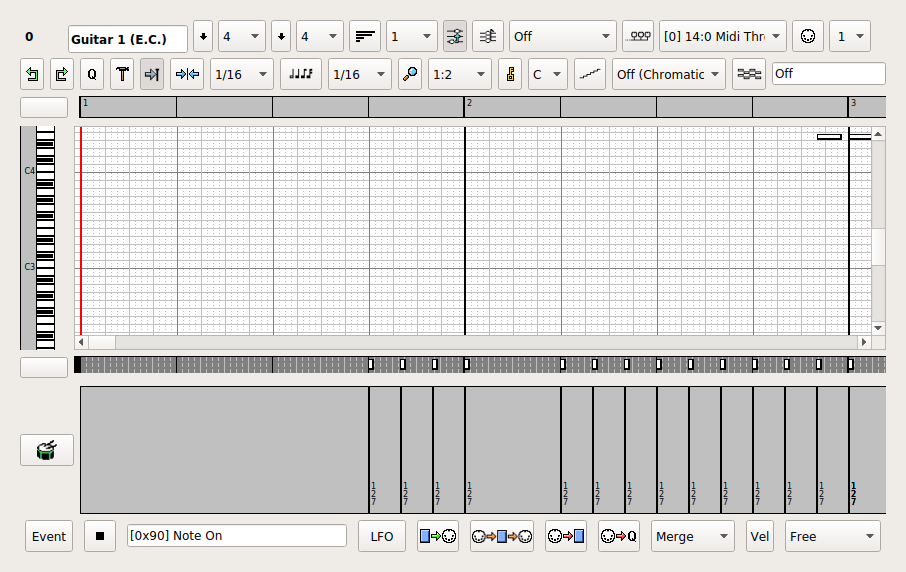
\includegraphics[scale=0.65]{roll.png}
   \caption{Currently-Edited Pattern, Unarmed}
   \label{fig:pattern_window_current_seq_unarmed}
\end{figure}

   If the currently-edited sequence is armed (unmuted), then the highlighting
   is reversed (cyan text on a black background), and resembles the
   highlighting for an armed sequence (which is white text on a black
   background).

\begin{figure}[H]
   \centering 
%  \includegraphics[scale=0.75]{pattern-window-current-seq-armed.png}
   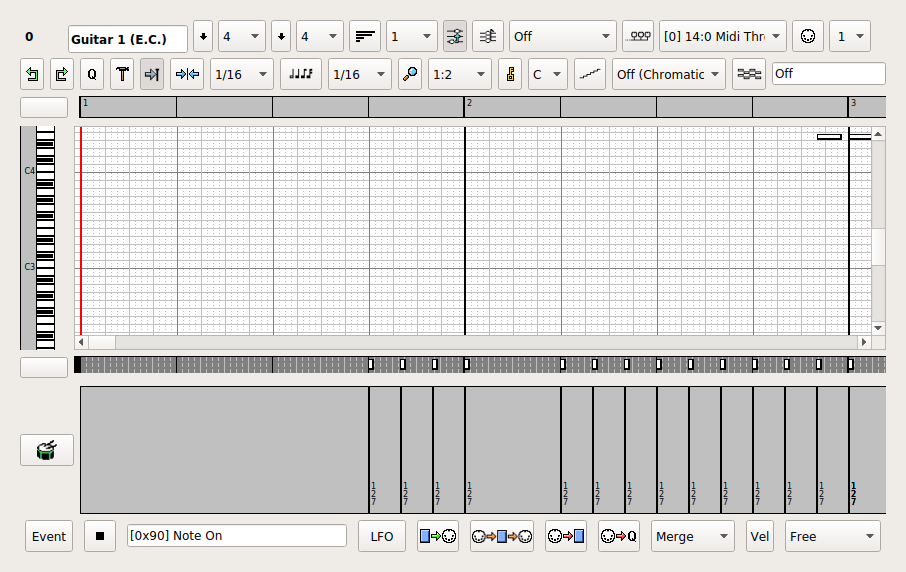
\includegraphics[scale=0.65]{roll.png}
   \caption{Currently-Edited Pattern, Armed}
   \label{fig:pattern_window_current_seq_armed}
\end{figure}

   If more than one sequence or \textbf{Event Editor}
   is brought up, only the slot for
   the last one to have focus is hightlighted.
   Note that this highlighting also applies to the \textbf{Event Editor}.

   \itempar{Paste}{pattern!paste}
   Pastes a loop or pattern that was previously copied.
   Also note that there is no \texttt{Ctrl-V} key for this operation in the
   main window.

   \itempar{Song}{pattern!song}
   The \textbf{Song} items are described later, in reference to
   \figureref{fig:pattern_window_right_click_song}.
   
\subsubsection{Pattern}
\label{subsubsec:seq66_patterns_pattern_filled}

   A filled pattern slot is referred to as a \textsl{pattern}
   (or \textsl{loop}, or \textsl{sequence}).
   A pattern is shown in the Pattern window as a filled box with the
   following items of information in it.
   Examine \figureref{fig:pattern_window_main_panel_items}; it shows
   these items annotated for clarity.

   \begin{itemize}
      \item \textbf{Name}.
         \index{pattern!name}
         This line contains the name or title of the pattern, to help
         reference it when juggling a number of patters.
      \item \textbf{Pattern Length}.
         \index{pattern!length}
         If the option to show pattern hot-key is enabled, the length of the
         pattern, in measures, is shown in the upper right corner of the
         pattern slot.  This feature is useful when recording tempo events that
         will increase the length of the tempo track.
      \item \textbf{Contents}.
         \index{pattern!contents}
         The contents of the pattern provide a fairly detailed and
         distinguishable representation of the notes or events in the
         pattern.  Also, when the song is playing, a vertical bar cursor
         tracks the position of the playback of the pattern or loop; it
         returns to the beginning of the box every time that pattern starts
         over again.
         \index{empty pattern}
         With \textsl{Sequencer66}, an imported empty pattern will no longer
         needlessly scroll.
         However, if a pattern has even a single event (say, a program change),
         it will scroll.
%        \textbf{TODO:}
%        \index{todo:one-shot pattern}
%        It might be good to have some patterns marked as one-shot patterns.
%        They play once at the start of playback, and that is it.
%        They could be marked with a cyan background.
%        Currently, it is easy enough to use the Song Editor for this purpose,
%        but then one cannot play the patterns in live mode.
      \item \textbf{Sequence Number}.
         If the option to show the sequencer number is set
         in the \textbf{File / Options / Keyboard} section
         (see \sectionref{paragraph:seq66_menu_file_options_keyboard},
         the this number is shown at the bottom left of the pattern slot.
      \item \textbf{Bus-Channel}.
         \index{pattern!bus-channel}
         This pair of numbers shows the the MIDI buss number, a dash, and
         the MIDI channel number.
         For example, "0-2" means MIDI buss 0, channel 2.
      \item \textbf{Beat}.
         \index{pattern!beat}
         This pair of numbers is the standard time-signature of the pattern,
         such as "4/4" or "3/4".  The first number is the beats-per-measure,
         and the second is the size of the beat, here, a quarter note.
      \item \textbf{Shortcut Key}.
         If the display of hot-keys is enabled (see
         \sectionref{paragraph:seq66_menu_file_options_keyboard}),
         then the key noted in the lower-right corner of the pattern can be
         pressed to toggle the mute/unmute status of that pattern.
         This action is an alternative to left-click on the pattern.
      \item \textbf{Progress Cursor}.
         At the left of each box is a vertical line, waiting for playback to
         start so that it can move through the pattern, again and again.
      \item \textbf{Armed}.
         See \figureref{fig:pattern_window_main_panel_items}; it shows a black
         and white pattern.  The black color indicates that the pattern is armed
         (unmuted), and will play if playback is initiated in the pattern
         \index{live mode}
         window in live mode.
         An item is armed/disarmed by a left-click on it.
         \index{shift left click}
         If the Shift key is held during a left-click on a pattern, then
         the armed/unarmed state of every other active pattern is toggled.
         This feature is useful for isolating a single track or pattern.
      \item \textbf{Queued}.
         That same pattern also shows that it is queued, which means that it
         will toggle its playing status when the pattern next begins again.
      \item \textbf{Alternate font}.
         Later builds of \textsl{Sequencer66} are now built with a new font.
         See \figureref{fig:pattern_window_main_panel_items}.  It shows the new
         font. 
         The old font can be selected in the "user" configuration file, and is
         also selected automatically if \textsl{Sequencer66} is run in the
         \textsl{legacy} mode.
      \item \textbf{Sequence number}.
         Later builds of \textsl{Sequencer66} are now built with the option to
         also show the sequence number in the pattern box, if the "show
         sequence numbers" option is on.
         This option can be set in the "user" configuration file.
         See \figureref{fig:pattern_window_main_panel_items}.  It shows an
         example of the sequence number, using the new font.
   \end{itemize}

   \index{pattern!left click}
   Left-click on an filled pattern box will toggle the status of the
   pattern between muted (white background) and unmuted (black background).
   If the song is playing via the main window, toggling this status makes
   the pattern stop playing or start playing.  The armed status
   can also be toggled using hot-keys.

   If the \textbf{Song Editor} is the active window and was used to
   start the playback, the pattern boxes will toggle between the muted/unmuted
   states as the music plays, and the pattern is active or inactive at the
   point of playback.  (The \textbf{Song Editor} acts as a list of triggers).

   \index{pattern!right click}
   A right-click on an already-filled box brings up a menu
   to allow one to edit it, or perform a few other actions
   specified in the context menu.  Here is that menu:

\begin{figure}[H]
   \centering 
%  \includegraphics[scale=0.75]{pattern/pattern-right-click-menu.png}
%  \includegraphics[scale=0.75]{new/seqmenu_menus-gtk-qt-0_96.png}
   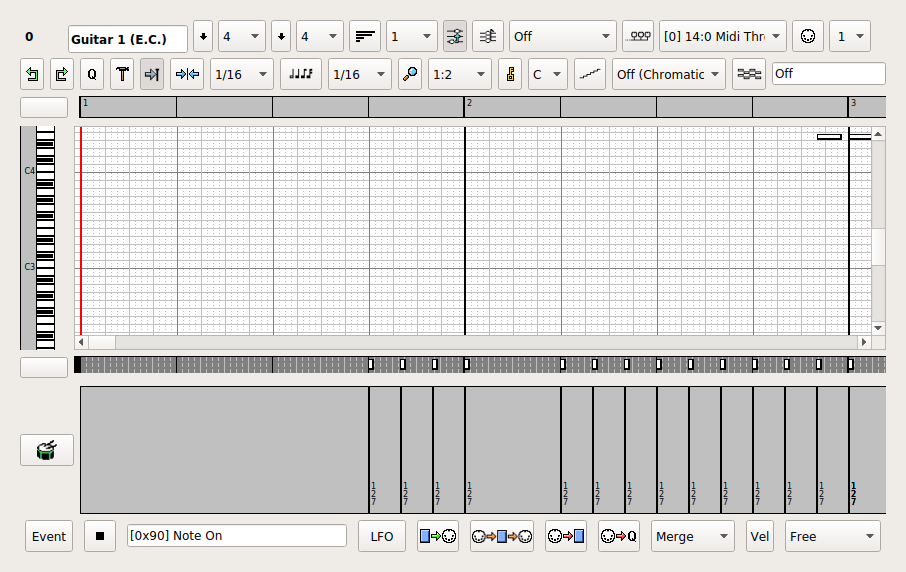
\includegraphics[scale=0.65]{roll.png}
   \caption{Existing Pattern, Right-Click Menus, Gtkmm and Qt Versions}
   \label{fig:pattern_window_right_click}
\end{figure}

   Here one can choose to edit the pattern, cut and copy the pattern,
   set the MIDI bus/channel, and more.
   One can also clear all performance (song) data for the pattern.
   Here are the Gtkmm menu entries:
   
   \begin{enumber}
      \item \textbf{Edit...}
      \item \textbf{Event Edit...}
      \item \textbf{Cut}
      \item \textbf{Copy}
      \item \textbf{Song}
      \item \textbf{Color}
      \item \textbf{Disable/Enable Transpose}
      \item \textbf{MIDI Bus}
   \end{enumber}

   The Qt menu entries are different and more extensive:
   
   \begin{enumber}
      \item \textbf{New pattern}
      \item \textbf{Extern live frame}
      \item \textbf{Edit pattern in tab}
      \item \textbf{Edit pattern in window}
      \item \textbf{Edit events in tab}
      \item \textbf{Set pattern color}
      \item \textbf{Copy pattern}
      \item \textbf{Cut pattern}
      \item \textbf{Delete pattern}
   \end{enumber}

   See \sectionref{subsubsec:qt_portmidi_qt5_live_slot_menu}.
   It describes these additional items and how the Qt user-interface works.
   The next sections describe the Gtkmm-accessible functions.

   \setcounter{ItemCounter}{0}      % Reset the ItemCounter for this list.

   \itempar{Edit...}{pattern!edit}
   Edits an existing loop or pattern.
   Clicking this menu entry brings up the \textbf{Pattern Editor}
   so that one can modify the existing pattern by click-dragging new notes in a
   piano roll user-interface.
   See \figureref{fig:pattern_edit_window}.
   Also known as the "sequence editor".

   In addition to right-click and selecting \textbf{Edit...}, the user can
   \index{empty slot double-click}
   double-click on the slot, to bring up the \textbf{Pattern Editor}.

   \index{pattern edit}
   \index{keys!=}
   \index{keys!pattern edit}
   Another way to bring up a pattern in the 
   \textbf{Pattern Editor} is to
   click the \textbf{equal} key and then the pattern's hot-key.
   For example, "\textbf{=q}" will open up the editor for the pattern with the
   hot-key \textbf{q}.
   The Equals key (\texttt{=}) is the default key that does this action.
   This key can be changed by modifying the
   \textbf{File / Options / Keyboard / Control keys / Pattern Edit} item.

   \itempar{Event Edit...}{pattern!event edit}
   \index{pattern event edit}
   Edits an existing loop or pattern, but using a detailed \textbf{Event Editor}
   that shows events as text and numbers, and allows editing them as text and
   numbers.
   See \figureref{fig:pattern_edit_window}.

   \index{event -}
   \index{keys!-}
   \index{keys!event edit}
   Another way to bring up the \textbf{Event Editor} is to
   click the \textbf{minus} key and then the pattern's hot-key.
   For example, "\textbf{-q}" will open up the \textbf{Event Editor}
   for that pattern.
   The Minus key (\texttt{-}) is the default key that does this action.
   This key can be changed by modifying the
   \textbf{File / Options / Keyboard / Control keys / Event Edit} item.

   The \textbf{Event Editor}
   is not the same as the \textbf{event} pane in the pattern
   editor; the \textbf{Event Editor} shows all events at once, and shows them
   only in text/list format.  This editor is basic, meant for viewing
   MIDI events and making some minor edits or deletes.
   The \textbf{Event Editor} is most useful when trying to find events
   that are screwing up the performance of that pattern.
   See \sectionref{sec:seq66_event_editor}, for more information.

   To simplify the application and avoid editing a pattern in
   two different dialogs, if either the 
   \textbf{Pattern Editor} or the
   \textbf{Event Editor} is
   active for a given sequence, the right-click sequence-slot menu leaves out
   the \textbf{Edit...} and \textbf{Event Edit...} menu entries.
   This trimmed menu looks like this:

\begin{figure}[H]
   \centering 
%  \includegraphics[scale=0.75]{pattern/pattern-right-click-menu-no-edit.png}
   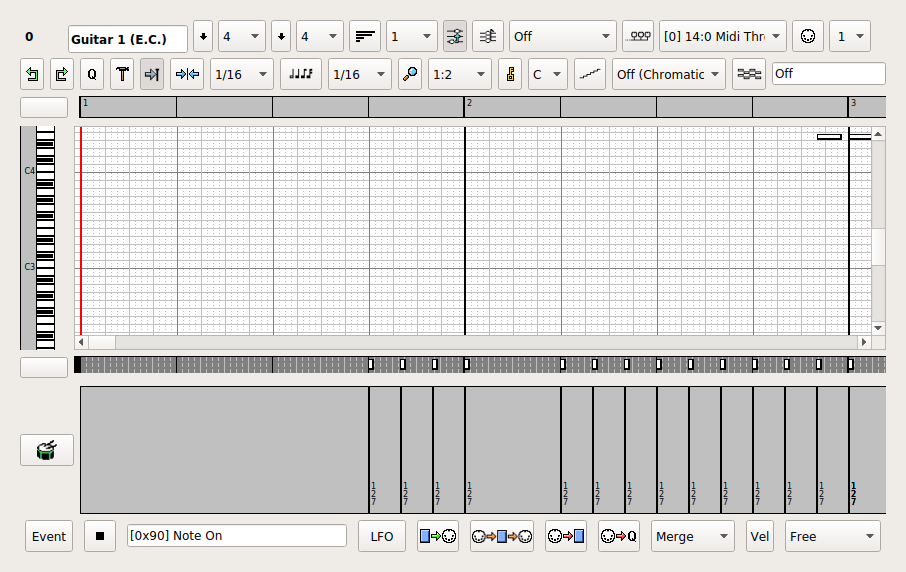
\includegraphics[scale=0.65]{roll.png}
   \caption{Existing Pattern, Right-Click Menu Without Edit Entries}
   \label{fig:pattern_window_right_click_no_edit}
\end{figure}

   The old functionality was to have the \textbf{Edit...} menu entry simply
   raise the existing 
   \textbf{Pattern Editor} to the top of the windows.

   \itempar{Cut}{pattern!cut}
   Deletes and copies an existing loop or pattern.
   One can also drag-and-drop a pattern into another cell (there is no outline
   box during the drag, sadly).
   Note that there is no \texttt{Ctrl-X} key for this operation in the
   main window.

% This bug was fixed:
%
%  \textbf{Bug:}
%  \index{bugs!pattern cut not dirty}
%  Although this operation works, it does not cause the user to be prompted if
%  the application is exited.

   \itempar{Copy}{pattern!copy}
   Copies an existing loop or pattern.
   The pattern can then be pasted elsewhere in the Patterns panel.
   One can also drag-and-drop a pattern into another cell (there is no outline
   box during the drag).
   See \sectionref{subsubsec:seq66_patterns_pattern_slot}.
   Note that there is no \texttt{Ctrl-C} key for this operation in the
   live (main) window.

   \itempar{Song}{pattern!song}
   Clicking this menu entry brings up a small popup menu:

\begin{figure}[H]
   \centering 
%  \includegraphics[scale=0.75]{pattern/pattern-menu-song.png}
%  \includegraphics[scale=0.75]{new/seqmenu_song_menu-0_9_15.png}
%  \includegraphics[scale=0.75]{new/seqmenu_song_menu-0_9_21.png}
   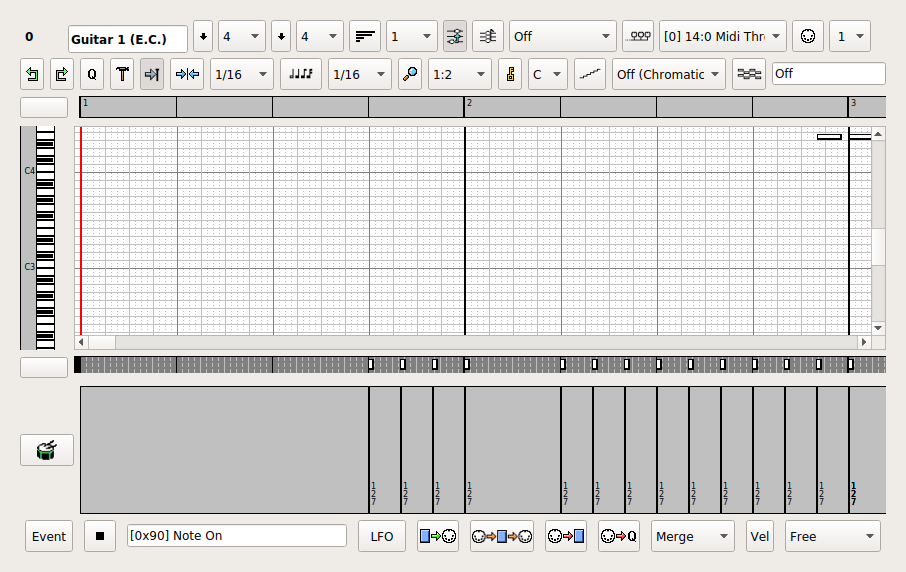
\includegraphics[scale=0.65]{roll.png}
   \caption{Existing Pattern, Right-Click Menu, Song}
   \label{fig:pattern_window_right_click_song}
\end{figure}

   \begin{enumber}
      \item \textbf{Clear This Track's Song Data}
      \item \textbf{Mute All Tracks}
      \item \textbf{Unmute All Tracks}
      \item \textbf{Toggle All Tracks}
      \item \textbf{Toggle Live Tracks}
   \end{enumber}

%  \setcounter{ItemCounter}{0}      % Reset the ItemCounter for this list.

   \index{Clear This Track's Song Data}
   \index{pattern!clear song data}
   \textbf{Clear This Track's Song Data}
   This item is not available if the pattern is empty.
   Selecting this filled-box right-click menu item causes that box's
   loop/pattern to be removed from the song editor.
   The triggers disappear from the Song Editor window, and so will not
   be played when the song plays in Song mode.

   \index{Mute All Tracks}
   \index{pattern!mute all tracks}
   \textbf{Song / Mute All Tracks}
   Selecting this filled-box right-click menu item causes
   the tracks in the Song Editor to be muted.  Sometime it takes a few seconds
   for the user-interfaces to show this big change.
   This item mutes all tracks (or loops/patterns).
   It works when one has opened the Song Editor window
   and started playing in playback
   mode by starting play using that window.

   So, let us assume the song is running in live (playback) mode.
   The patterns that are active (unmuted) in the live window are shown with a
   black background in the main patterns window.  If one right clicks on a
   pattern cell and selects \textbf{Song / Mute All Tracks}, all those patterns
   will become white and be silenced.  Eventually, the Song Editor window
   catches up and shows the "M" activated for all tracks.

   \index{Unmute All Tracks}
   \index{pattern!unmute all tracks}
   \textbf{Unmute All Tracks}
   Provides the opposite functionality, making all tracks armed and audible.
   Selecting this filled-box right-click menu item causes
   the tracks in the song to be unmuted.

   \index{Toggle All Tracks}
   \index{pattern!toggle all tracks}
   \textbf{Toggle All Tracks}
   Toggles the armed/mute status of all tracks.
   It doesn't matter if Live or Song Mode is in force.
   \index{keys!F8}
   By default, the \texttt{F8} key will also toggle all tracks.

   Note that there is also a feature where a
   \texttt{Shift-Left-Click} on a pattern slot toggles the mute
   status of the \textsl{other tracks}.

   \index{Toggle Live Tracks}
   \index{pattern!toggle live tracks}
   \textbf{Toggle Live Tracks}
   Toggles the mute status of only the armed/unmuted tracks when in Live mode.
   Works only in Live mode.  This operation unmutes all tracks that are
   currently unmuted.  The statuses of these armed tracks are saved; when
   this operation is performed again, those tracks are unmuted, turned back on.
   This menu entry provides the same function as the \textbf{Mute}
   button in the main window.

   \itempar{Color}{pattern!color}
   This menu item allows for specifying colors for the patterns.
   Colors can make it easier to find a pattern while running live.
   Note that there are some minor issues with colors, and that this feature is
   still in flux.

   \itempar{Enable/Disable Transpose}{pattern!transpose}
   This menu entry changes depending upon whether the new transpose feature is
   enabled or disabled for the sequence/pattern.  Note that, if the events
   shown in the slot are red, this denotes that transpose is currently
   \textsl{disabled} for that pattern, which might be a drum pattern.

   \itempar{MIDI Bus}{pattern!midi bus}
   Selecting this filled-box right-click menu item brings up a list
   of the up to 16 MIDI output busses that \textsl{Sequencer66} supports.
   For each of these buss items, another pop-up menu allows one
   to specify the MIDI output channel for that buss.

% \begin{figure}[H]
%  \centering 
%  \includegraphics[scale=0.65]{pattern/pattern-menu-midi-bus.png}
%  \caption{Existing Pattern, Right-Click Menu, MIDI Output Busses}
%  \label{fig:pattern_window_right_click_midi_bus}
% \end{figure}

\begin{figure}[H]
   \centering 
%  \includegraphics[scale=0.75]{pattern/pattern-menu-midi-bus-port.png}
   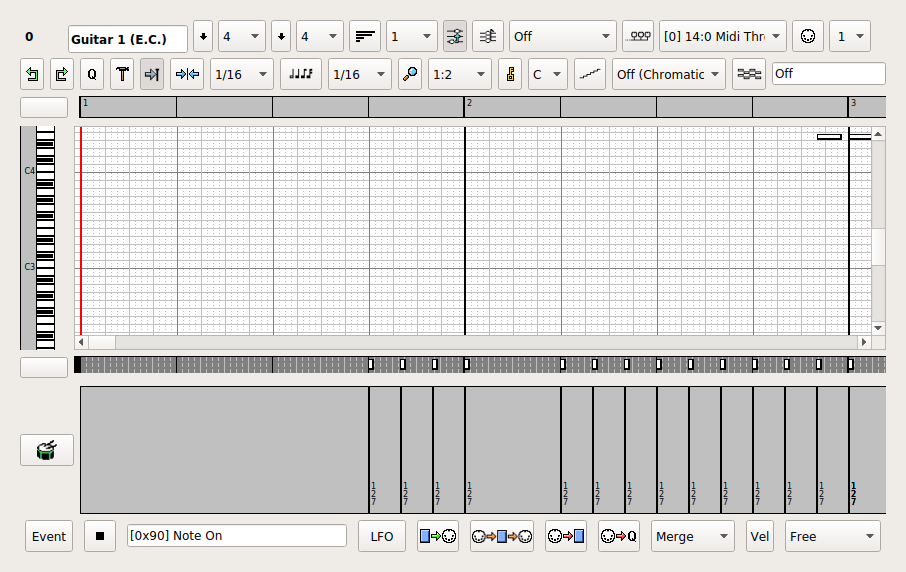
\includegraphics[scale=0.65]{roll.png}
   \caption{Existing Pattern Right-Click Menu, MIDI Output Busses/Channels}
   \label{fig:pattern_window_right_click_midi_bus}
\end{figure}

   \index{--bus option}
   Another way to specify busses is the
   \texttt{--buss n} command-line option.
   It causes \textsl{every} pattern in the MIDI
   file to be directed to that buss number, and when a new
   sequence/pattern is created.  This option is only
   for convenience in testing.  Save the file, and it will
   have that buss number as part of each track's data, which makes the song
   file less portable, so be careful.

% \begin{figure}[H]
%  \centering 
%  \includegraphics[scale=0.65]{pattern/pattern-menu-midi-bus-numbers.png}
%  \caption{Existing Pattern, Right-Click Menu, MIDI Buss Channels}
%  \label{fig:pattern_window_right_click_midi_bus_numbers}
% \end{figure}

\subsubsection{Pattern Keys and Click}
\label{subsubsec:seq66_patterns_pattern_keys_and_clicks}

   This section recapitulates all the clicks and keys that perform actions
   in the Pattern windows.  Some additional clicks and keys are noted here
   as well.

\paragraph{Pattern Keys}
\label{paragraph:seq66_patterns_pattern_keys}

   \index{keys!hot}
   \index{keys!shortcut}
   Each pattern in the patterns panel can have a hot-key or shortcut-key
   associated with it.

   \index{keys!pattern toggles}
   For each pattern, hitting its assigned hot-key will
   also toggle its status between muted/unmuted (armed/unarmed).
   Below is the default grid that is
   mapped to the loops/patterns on the screen-set.
   This grid can be changed in the
   \textbf{File / Options / Keyboard} tab, and is
   saved in the \textsl{keyboard-control} section of the
   \index{rc file}
   "rc" file.

   \begin{verbatim}
      [ 1 ][ 2 ][ 3 ][ 4 ][ 5 ][ 6 ][ 7 ][ 8 ]
      [ q ][ w ][ e ][ r ][ t ][ y ][ u ][ i ]
      [ a ][ s ][ d ][ f ][ g ][ h ][ j ][ k ]
      [ z ][ x ][ c ][ v ][ b ][ n ][ m ][ , ]
   \end{verbatim}

   These characters are shown in the lower right corner of each
   pattern, as an aid to memory.

   A "shift" functionality is available for the
   mute/unmute hot-keys when a set is larger than 32 patterns.
   \index{variset!slash key}
   Normally, pressing the \texttt{1} key will toggle
   sequence 0.  If preceded by one slash key (\texttt{/}), then sequence 32
   will be toggled.  If preceded by two slash keys, then sequence 64 will be
   toggled.  This features supports using set sizes of 32, 64, and 96 patterns.

\begin{figure}[H]
   \centering 
%  \includegraphics[scale=0.50]{new/patterns_panel_shift_toggle.png}
   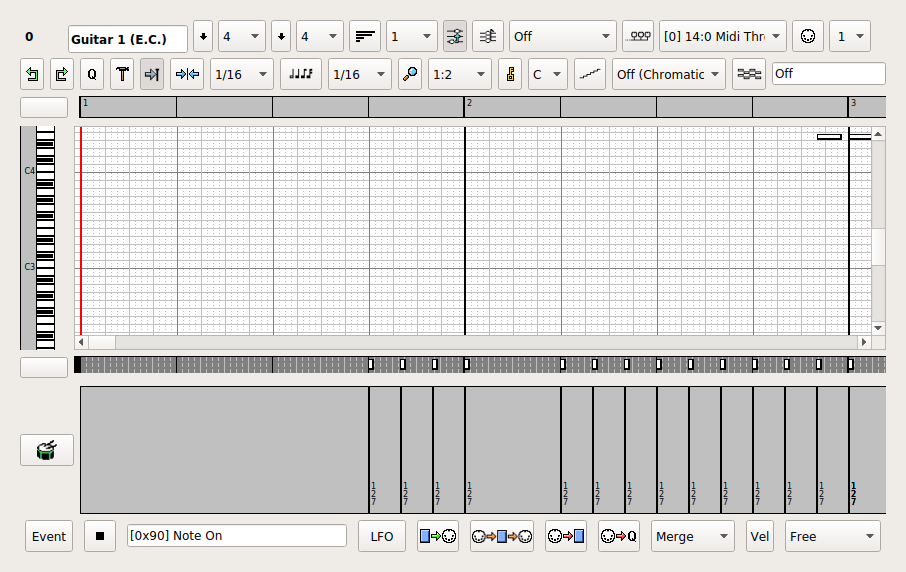
\includegraphics[scale=0.65]{roll.png}
   \caption{Patterns Panel, Shift-Key Pattern Toggle}
   \label{fig:pattern_window_shift_key_pattern_toggle}
\end{figure}

   This figure shows how one presses \texttt{y}, \texttt{/y}, and \texttt{//y}
   to arm three patterns in this 96-pattern set.

   \index{keys![}
   \index{keys!decrement set}
   \index{keys!screenset down}
   The "\texttt{[}" and
   \index{keys!]}
   \index{keys!increment set}
   \index{keys!screenset up}
   "\texttt{]}" keys on the keyboard decrement or increment the set number.

   \index{keys!alt}
   \index{keys!snapshot}
   The left and right \texttt{Alt} keys are, by default, set up in the
   \textbf{File / Options / Keyboard / Snapshot 1} and
   \textbf{Snapshot 2} fields to be used as "snapshot" keys.
   Our preference is to use something that does not trigger desktop
   commands, perhaps "\texttt{F11}" or "\texttt{F12}", or one of the keys in
   the keypad.

   When a snapshot key is pressed, the state of the patterns
   (armed versus unarmed) is saved.  While the
   snapshot key is held, one can then change the state of the patterns
   (using the keyboard, \textsl{not} the mouse)
   to change how the song plays.  When the snapshot key is released, the
   original saved state of the patterns is restored.

%  \index{keys!alt}
%  \index{keys!snapshot}
%  Holding \texttt{Alt} will save the state of playing patterns and restore
%  them when \texttt{Alt} is lifted.
%  The handling of \texttt{Alt} is often taken over by the application,
%  so there could be a need to change these items to some other
%  keys.  For example, we have the \textsl{Fluxbox} window manager
%  set up so that the \texttt{Alt} keys can
%  be used for moving or resizing a window.  Therefore, we use
%  keypad keys for this purpose.

%  \index{keys!left ctrl alt}
%  Holding \texttt{Left Ctrl} and \texttt{Alt} at the same time will enable
%  one to flip over to new patterns briefly and then flip right back upon
%  lifting \texttt{Alt}.  Not yet sure exactly what this means.

   \index{keys!right ctrl}
   \index{keys!queue}
   \index{queue!temporary}
   Holding the "queue" key and then hitting a pattern hot-key
   will queue an on/off toggle for a pattern when the end of the loop is
   reached.
   This is the "queue" functionality.
   This means that the change in state of the pattern will not take hold
   immediately, but will kick in when the pattern restarts.
   This pending state is indicated by coloring the central box of the
   pattern grey, as shown in the figure below.
%  Note that queuing can also be used to turn a pattern \textsl{off}
%  at the end of a pattern.
   Please note the "keep queue" functionality and
   the "one-shot queue" functionality described below.

\begin{figure}[H]
   \centering 
%  \includegraphics[scale=0.75]{pattern/seq24-queueing-coloration.jpg}
%  \includegraphics[scale=0.75]{new/seq66-queueing-coloration.png}
   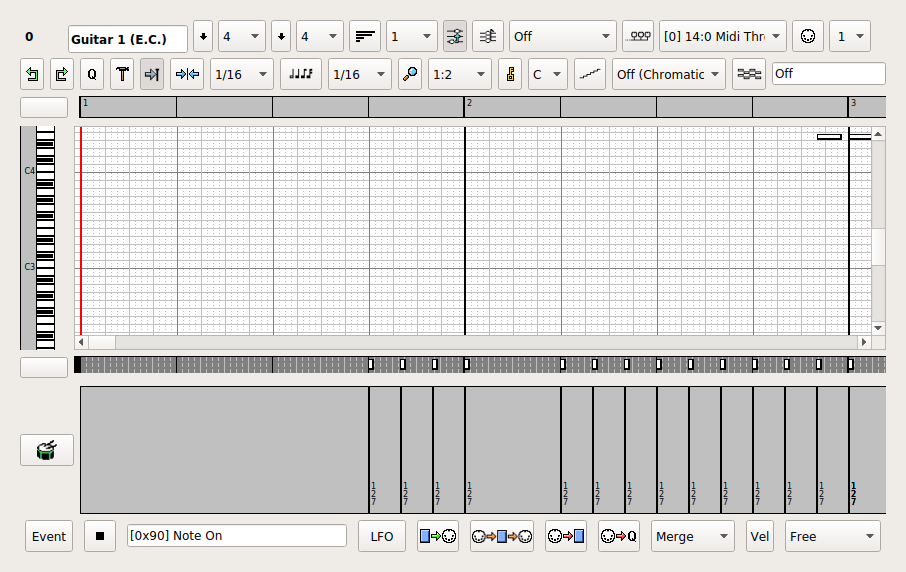
\includegraphics[scale=0.65]{roll.png}
   \caption{Pattern Coloration when Queued}
   \label{fig:seq66_queueing_coloration}
\end{figure}

   This figure shows the coloring for queuing in the top two patterns with
   dark grey event backgrounds.  At the end of the pattern, the left top
   pattern will turn off, and the right top pattern will turn on.
   The bottom two patterns show the light-grey coloring used to show
   a "one-shot" queue.  The one-shot queue can only turn a pattern on, and it
   will force the pattern off after one play.
   Queue also works for mute/unmute pattern sets ("groups"); in this case,
   every sequence will toggle its status after its individual loop ends. 

   \index{keys!avoid ctrl/alt}
   We do \textbf{not}
   recommend using \texttt{Ctrl} or \texttt{Alt}
   keys for pattern control.  They conflict with application or desktop
   settings.  However, if one insists on such hot-key combinations,
   use the \textbf{Menu} button in the main
   window to disable the menu.
   One can also use normal keys to enable queuing.
   For example, the minus key or the keypad's slash key can be used.
%  , which makes those keystrokes more
%  safely available.
%  The \texttt{Super} key can also be used, if not already used by the desktop
%  environment.  Also available are some of the function keys, and, if
%  available, the keypad keys.  These can be configured in
%  \textbf{File / Options / Keyboard} and
%  \textbf{File / Options / Ext Keys}.
%  Of course, if the \texttt{Ctrl} key is used to manage the GUI (e.g.
%  \texttt{Ctrl-Q} will unceremoniously quit the application), so one will
%  usually want to change this key to something else in the
%  \textbf{File / Options / Keyboard / Queue} field.
%  The \texttt{Super} key (i.e. the \texttt{Mod4} or \texttt{Windows key}) is a
%  good candidate to substitute for the \texttt{Ctrl} key, unless one has (like
%  the author)
%  configured the window manager to use the \texttt{Super} key to manipulate
%  windows and applications \textsl{(laughter ensues)}.
%  , with no flickering due to the keyboard repeat rate.

   \index{keys!keep queue}
   \index{queue!keep}
   Pressing the "keep queue" hot-key
   \index{rc file}
   assigned in the "rc" file activates a "sticky" queue mode.
   In this mode, pressing a pattern key immediately turns on queuing, instead
   of mute/unmute.  And multiple patterns can be handled in this way at the
   same time.
   Keep-queue persists until one clicks the normal queue function hot-key,
   or changes the active (viewed) screen-set. 
%  After pressing the "keep queue" hot-key, individual pattern
%  toggles are queued rather than happening immediately.
%  While in queue mode, pressing a patterns hot-key, or clicking on the
%  pattern, queues that pattern to change state at the beginning of the next
%  loop.
   \index{queue!cancel}
   “Keep queue” mode is cancelled by pressing the normal queue hot-key.
   This hot-key can be changed in the
   \textbf{File / Options / Keyboard / Keep queue} field.
   There is also a \textbf{Q} button for the same purpose.
   Also note the "queued replace/solo" functionality, described a bit later.

   \index{one-shot queue}
   \index{keys!one-shot queue}
   \index{queue!one-shot}
   Thanks to \textsl{Kepler34}, we have "one-shot queue"
   functionality.  This one-shot setup queues a pattern up for unmuting only,
   and, once the pattern has played, it is automatically muted.  This process
   is easier than having to unqueue the pattern manually before the next
   playback.
   This hot-key can be changed in the
   \textbf{File / Options / Ext Keys / One-shot queue} field.

   \index{keys!replace}
   The "replace" hot-key (the left \texttt{Ctrl} key by default, which 
   should be changed to something better), 
   sets a form of muting/unmuting.  When the "replace" hot-key is
   pressed and held while clicking a pattern or pressing that pattern's
   hot-key, that sequence is unmuted, and all of the other sequences are muted.
%  Again, \texttt{Ctrl}
%  is a very inconvenient default, so an alternative key mapping
%  should be set up in the "rc" file via the \textbf{File / Options / Keyboard}
%  tab.
   "Replace" is a form of "solo".
   "Replace" is also implemented via MIDI control,
   where the MIDI control can be activated, but then the user has to select
   the desired sequence.  

   \index{queue!replace}
   \index{queue!solo}
   \textsl{Sequencer66} provides an extension to the replace/solo functionality
   that is called "queued-replace" or "queued-solo".  In this feature, when
   the "keep queue" function is activated, the replace function is queued so
   that it does not occur until the next time the patterns loop.
   And queued-replace provides a form of snapshot, limited to the
   \textsl{current} screen-set.
   Here are the steps:

   \begin{enumber}
      \item Start playback with some patterns on. 
      \item Press and release
         the "keep queue" hot-key.  This puts the application into "queue" mode.
         It is indicated via a "\textbf{Q}" button.
      \item Press and hold the "replace" hot-key.
      \item Click the desired pattern hot-key.  Observe that it arms or
         stays on, and that the other playing patterns show the "queued" color
         (grey).  At the end of the loop, they turn off, and the "replace"
         pattern is now solo.
      \item Click the same pattern hot-key again.  Observe that the other
         patterns that were toggled off are now queued to be toggled on at the
         next loop.  Steps 4 and 5 can be repeated endlessly.
      \item To end
         \index{queue!clear}
         \index{queue!end}
         the "queued-replace" mode, click the normal "queue"
         hot-key.  Also, changing the active screen-set ends "queue-replace"
         mode.  It does \textsl{not} end normal queue mode, to preserve the
         behavior found in \textsl{Seq24}.
         One needs to clear the queue mode in order to select another pattern
         to solo.
   \end{enumber}

\begin{figure}[H]
   \centering 
%  \includegraphics[scale=0.75]{new/queued_replace.png}
   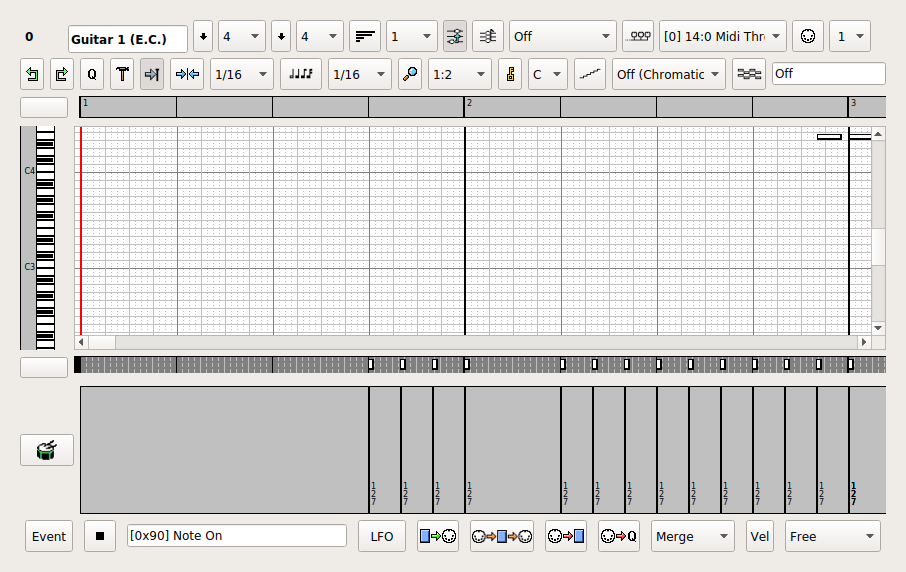
\includegraphics[scale=0.65]{roll.png}
   \caption{Queued-Replace (Queued-Solo) In Action}
   \label{fig:queued_replace}
\end{figure}

   Before pressing the "keep queue" key, patterns 33 ("\textbf{q}")
   and 34 ("\textbf{a}") are
   unmuted, while the desired replace pattern, 32 ("\textbf{1}") is off.
   Then the user presses (and holds) the "replace" key, then clicks the
   "\textbf{1}" key.
   This puts all unmuted patterns, plus the muted
   replace pattern as well, into queue mode, as shown by the grey panels.
   When the progress bar reaches the end of the pattern, pattern 32 will go on,
   and patterns 33 and 34 will go off.
   If the replace-pattern is already on, it is not queued, as
   there's no need to turn it on.

   If, while in queue mode, the replace key is held and
   "\textbf{1}" is pressed again,
   the other patterns will be queued, and will turn on again.  Thus, the
   solo status of the replace pattern can be toggled at will, until queue mode
   is exited by pressing and releasing the normal "queue" key.
   If the replace key is \textsl{not} held down, and another pattern's replace
   hot-key is pressed, that pattern will be queued normally.
   If one wants to change the solo functionality to a different pattern,
   simple hold the replace key and click on a different pattern.  The new
   arrangement of soloing is memorized.
   One can clear the queue mode by pressing the normal queue key.

   There are more keys defined in the \textbf{Keyboard} dialog, and it is
   worth figuring out what they do, if not documented here.
   For a couple of short, but good, video tutorials about using arming,
   queuing, and snapshots, see references \cite{wootangent1}
   and \cite{wootangent2}.

   \index{solo!true}
   \index{pattern!shift-left-click}
   \index{patterns panel!inverse muting}
   \index{patterns panel!solo}
   \index{shift-left-click solo}
   There is a truer "Solo" functionality in the Patterns
   Panel and the Song Editor.  To "solo" a pattern, move the mouse cursor
   over the pattern, hold the \texttt{Shift} key, and left-click the pattern.
   This will turn off all the other patterns, so that the selected pattern ins
   the only one playing.  Holding the \texttt{Shift} key and clicking the same
   pattern again will unmute all of the other patterns.

\paragraph{Pattern Clicks}
\label{paragraph:seq66_patterns_pattern_Clicks}

   \index{pattern!left click}
   \index{pattern!mute toggle}
   Left-click on a pattern-filled box will change its state
   \index{pattern!mute}
   \index{pattern!unmute}
   from muted (white background) to playing (black background), whether
   the sequencer is playing or not.

   \index{pattern!left click-drag}
   Left-click-hold-drag on a pattern, drags it to a different
   pattern on the grid.
   The box disappears while dragged, and reappears in the new location when
   dropped.  However, a pattern \textsl{cannot} be dragged if its
   \textbf{Pattern Editor} window is open.

   \index{pattern!right click}
   Right-click on a pattern brings up the appropriate context menus, as
   discussed earlier, depending on whether the pattern box is empty or
   filled.

   \index{pattern!middle click}
   Middle-click does nothing when the mouse rests inside a pattern box.

\subsection{Patterns / Bottom Panel}
\label{subsec:seq66_patterns_panel_bottom}

   The bottom panel of the Patterns window provides way to control the
   overall playback of the song.  It has changed quite a bit over the last few
   versions of \textsl{Sequencer66}, and we have not yet caught up with the
   diagrams. And the Qt user-interface adds more changes.
   Refer to the diagram of the whole window, for now.

\begin{figure}[H]
   \centering 
%  \includegraphics[scale=0.75]{pattern-window-bottom-panel-items.png}
%  \includegraphics[scale=0.50]{new/pattern-window-bottom-panel.png}
   \includegraphics[scale=0.65]{roll.png}
   \caption{Patterns Panel, Bottom Panel Items}
   \label{fig:pattern_window_bottom_panel_items}
\end{figure}

   This figure shows a number of new items.

   \begin{enumber}
      \item \textbf{Panic!}
      \item \textbf{Stop}
      \item \textbf{Play and Pause}
      \item \textbf{Song Record}
      \item \textbf{Song Record Snap}
      \item \textbf{BPM}
      \item \textbf{Tap Tempo}
      \item \textbf{Log Tempo}
      \item \textbf{Record Tempo}
      \item \textbf{Keep-Queue Status}
      \item \textbf{Name}
      \item \textbf{Set}
      \item \textbf{Toggle Song Editor}
   \end{enumber}

   \setcounter{ItemCounter}{0}      % Reset the ItemCounter for this list.

   \itempar{Panic!}{pattern!panic}
   This new button stops the song and sends MIDI Off messages on all notes.

   \itempar{Stop}{pattern!stop}
   The red square button stops the playback of the song and all its patterns.
   \index{keys!esc (stop)}
   The keystroke for stopping playback is the \texttt{Escape} character.
   It can be changed to \texttt{Space}, so that the space-bar then becomes
   effectively a playback toggle key.

   \itempar{Play and Pause}{pattern!Play}
   \index{pattern!Pause}
   The green triangular button starts the playback of the whole song.
   \index{keys!space (play)}
   The keystroke for starting playback is the \texttt{Space} character by
   default.

   \index{pause}
   The Play button can be used as a Pause button.
   When the Play button is clicked, the button icon changes to a Pause icon:

\begin{figure}[H]
   \centering 
%  \includegraphics[scale=1.0]{new/stop_pause_buttons.png}
   \includegraphics[scale=0.65]{roll.png}
   \caption{Patterns Panel, Pause Button}
   \label{fig:pattern_window_pause_button}
\end{figure}

   A Pause key (by default, the period) is also defined.
%  (The pause feature can be removed by rebuilding the application
%  after configuring with the \texttt{--disable-pause} option.)

   \itempar{Song Record}{pattern!song record}
   Song-recording in \textsl{Sequencer66} is adopted from the
   \textsl{Kepler34} project.
   This feature takes live muting changes and records them as
   triggers in the \textbf{Song Editor}.
   The default hot-key for this function is \texttt{P}.
   This feature does not honor queuing...
   rather than waiting until the end of the pattern when the queuing takes
   effect, the trigger recording starts immediately.

   \itempar{Song Record Snap}{pattern!song record snap}
   This button toggles snapping the beginning and end of a recorded trigger to
   the nearest beat.  There is no hot-key for this button at this time.

   \itempar{BPM}{pattern!BPM}
   The spin widget adjusts the "beats per minute" (BPM) value.  The
   range of this field is from 1 bpm to 600 bpm, with a default value of
   120 bpm.
   Although this field looks editable, it is not.  Most keystrokes
   that are entered actually toggle one of the pattern boxes.
   However, the following keys can also modify the BPM in small increments:
   \index{keys!semicolon}
   The \texttt{semicolon} reduces the BPM;
   \index{keys!apostrophe}
   The \texttt{apostrophe} increases the BPM.
   Also, if one right-clicks on the Up button, the BPM advances to its largest
   supported value, and if one right-clicks on the Down button, the BPM
   advances to its lowest value.
   MIDI control for this value is also available.

   The precision of the BPM value can be set to 0, 1, or 2
   decimal places, and the increment values for the step size (small)
   or page size (large) of the BPM spinner can be configured in the "usr" file.
   See \sectionref{subsec:seq66_usr_file_user_midi_settings}; it describes
   the precision and increment options more fully.
   The following figure shows the appearance of the BPM field with different
   precision values:

\begin{figure}[H]
   \centering 
%  \includegraphics[scale=0.65]{new/bpm_precision_settings.png}
   \includegraphics[scale=0.65]{roll.png}
   \caption{Patterns Panel, BPM Precisions}
   \label{fig:pattern_window_bpm_precision_settings.png}
\end{figure}

   \itempar{Tap Tempo}{pattern!tap tempo}
   This control is clicked in time with a tune, to set the
   tempo based on the tempo of the clicks.  Once clicked, the label of this
   button increments with every click, and the \textbf{BPM} field updates to
   display the calculated tempo.  If the user stops tapping for 5 seconds, the
   label reverts to 0, the BPM value keeps its final value, and the user can
   try tapping the tempo again, or accept the current value.
   Tapping can also be done using the keystroke defined
   in \textbf{File / Options / Ext Keys / Tap BPM}.
   It defaults to the "\texttt{F9}" key.

   \itempar{Log Tempo}{pattern!log tempo}
   This light-magenta button (Gtkmm only),
   logs the current tempo at the
   current playback spot as a Set Tempo meta-event, in the first
   track (pattern slot \#0) or the alternate tempo track if defined,
   and only if it is active.  According to the MIDI standard, such events
   should be present \textsl{only} in the first track,
   and so \textsl{Sequencer66} follows this rule, and also makes tempo events
   officially supported.  They can be edited in the 
   \textbf{Pattern Editor} or in the
   \textbf{Event Editor}.
   The main/global tempo is not written to the tempo track; it is stored in
   a SeqSpec section.
   See \sectionref{sec:meta_events}, for more information.

   \itempar{Record Tempo}{pattern!record tempo}
   This dark-magenta button (Gtkmm only)
   becomes light-magenta when activated, and turns on
   the recording of any tempo changes made in the BPM spinner.  If the spinner
   is held down, a ramping stream of tempo events is created.  If
   the time exceeds the current length of the tempo track, then the length of
   the track is automatically increased.
   These tempo events will not affect playback speed
   unless the tempo track is unmuted.

   \itempar{Keep-Queue Status}{pattern!keep-queue}
   This item is the \textbf{Q} button.
   It provides a visual way to know the current state of keep-queue, and is
   activated either by clicking on it or by pressing the assigned keep-queue
   key.

   \itempar{Name}{pattern!set name}
   Each of the 32 available screen-sets can be given a name by entering it
   into this field.  This name is saved with the MIDI file.

% This bug is fixed, as of 0.9.18, IIRC
%
%  \textbf{Bug:}
%  \index{bugs!set name has side-effect}
%  While one is typing in the name of the set in this field, the keystrokes
%  will affect the panel window, causing playback to start and pattern
%  boxes to be toggled!

   \itempar{Set}{pattern!set number}
   This spin widget selects the current screen-set.  The values in this
   field range from 0 to 31 (less if the set-size is a larger value),
   and default to 0.
%  Although this field looks editable, it is not.

% This bug is fixed, as of 0.9.18, IIRC
%
%  \textbf{Bug:}
%  \index{bugs!set number has side-effect}
%  While one is typing in the number of the set in this field, the keystrokes
%  will affect the panel window as well.

   \itempar{Toggle Song Editor}{pattern!toggle song editor}
   Pressing this button toggles the presence on-screen of the
   \textbf{Song Editor}.  The \texttt{Ctrl-E} keystroke can also be used.

\subsection{Patterns / Multiple Panels}
\label{subsec:seq66_patterns_panel_multiple}

%  If \textsl{Sequencer66} is built with the \texttt{--enable-multiwid}
%  \textsl{Sequencer66} has a "multiwid" option, this defines the 
%  \texttt{SEQ64\_MULTI\_MAINWID} macro, and allows for
   \textsl{Sequencer66} has a "multiwid" option, which
   allows for
   \index{multi-wid}
   multiple live panels showing more than one set at a time.
   The default is to show the usual single "mainwid".
   In the Qt user-interface, multiple live panels in separate windows
   can be opened.

\begin{figure}[H]
   \centering 
%  \includegraphics[scale=0.50]{multiwid/multiwid-mode-3x2.png}
   \includegraphics[scale=0.65]{roll.png}
   \caption{Patterns Panel, with Multiple Panels}
   \label{fig:pattern_window_bottom_panel_multiple}
\end{figure}

   In the Gtkmm user-interface, either one spinner for all, or one spinner for
   each, is available.  The latter is the "independent" mode.
   Note that it is possible, in this mode, to show the same set in two
   different "mainwids", but this is not recommended, as there may be minor
   unavoidable issues with that.

   Note that Page Up and Page Down keystrokes, as well as their
   configurable counterparts in
   \textbf{File / Options / Keyboard / Control Keys / Screenset Up}
   and \textbf{Screenset Down}, apply only to the top leftmost "mainwid".
   Of course, if the "mainwids" are synced, then all are affected by these
   keystrokes.

   In multi-wid mode, each "mainwid" frame shows the corresponding set number
   and, if present, the set notepad text for each "mainwid" set.

   See 
   \sectionref{sec:seq66_man_page}, for how the
   \texttt{-o wid=3x2,i} option can be used to set this mode, and
   \sectionref{subsec:seq66_usr_file_user_interface_settings}, for
   how these settings can be made permanent in the "usr" file.
   In that file, the options modified are \texttt{block\_rows} and
   \texttt{block\_columns}.

\subsection{Patterns / Variable Set Size}
\label{subsec:seq66_patterns_panel_variset}

   \index{variset}
   This option, informally known as "variset", allow some changes in
   the set size and layout from the default 4x8 = 32 sets layout.
   The row count can be set from 4 to 8, and the column count can be set to 8
   to 12.  Note that the set size can only be \textsl{increased} by these
   settings.

   \textbf{Warning:}
   \textsl{seq24} was fairly hardwired for supporting 32 patterns per
   set, and there are still places where that is true.  Thus,
   consider this option to be experimental.

   Also see 
   \sectionref{sec:seq66_man_page}, for how the
   \texttt{-o sets=8x8} option can be used to set this mode, and
   \sectionref{subsec:seq66_usr_file_user_interface_settings}, for
   how these settings can be made permanent in the "usr" file.
   In that file, the options modified are \texttt{mainwnd\_rows} and
   \texttt{mainwnd\_cols}.

\begin{figure}[H]
   \centering 
%  \includegraphics[scale=0.50]{multiwid/variset-mode-8x8.png}
   \includegraphics[scale=0.65]{roll.png}
   \caption{Patterns Panel, 8 x 8 Layout}
   \label{fig:pattern_window_bottom_panel_variset}
\end{figure}

   Generally, it is recommend to stick with the 4x8 (32 patterns/set),
   8x8 (64 patterns/set), and 8x12 (96 patterns/set).  This works best with the
   existing set of 32 hot-keys.

   Also note that the Qt 5 user-interface also supports "variset", whether in
   the main window or in the external live-frame.  In addition, both Qt windows
   can be resized and still show good renditions of the pattern-slots.

%-------------------------------------------------------------------------------
% vim: ts=3 sw=3 et ft=tex
%-------------------------------------------------------------------------------
